% An example of UML modeling

\documentclass[crop,border={10pt,10pt,10pt,10pt},tikz]{standalone}

%%%%%%%%%%%%%%%%%%%%%%%%%%%%%%%%%%%%%%%%%%%%%%%%%%%%%%%%%%%%%%%%%
\usepackage[]{pgf-umlcd}
\usepackage{tikz}
\usepackage{listings}
\usepackage{hyperref}
\usepackage{amsmath}
\usepackage{amssymb}
\usepackage{etoolbox}
\usepackage{amssymb}
\usepackage{xcolor}
\usepackage{pgfplots}
\usepackage{braids}
\usepackage{tkz-graph}
\usepackage{pgfplots}
\usepackage{amsbsy}
\usepackage{etoolbox}
\usepackage{color}
\usepackage{bm}
\usepackage{relsize}

\usetikzlibrary{arrows,decorations.pathmorphing,backgrounds,fit,petri,shadows}
\usetikzlibrary{automata, chains, decorations.pathmorphing, positioning}
\usetikzlibrary{patterns,calc,snakes,shapes,matrix}

\begin{document}
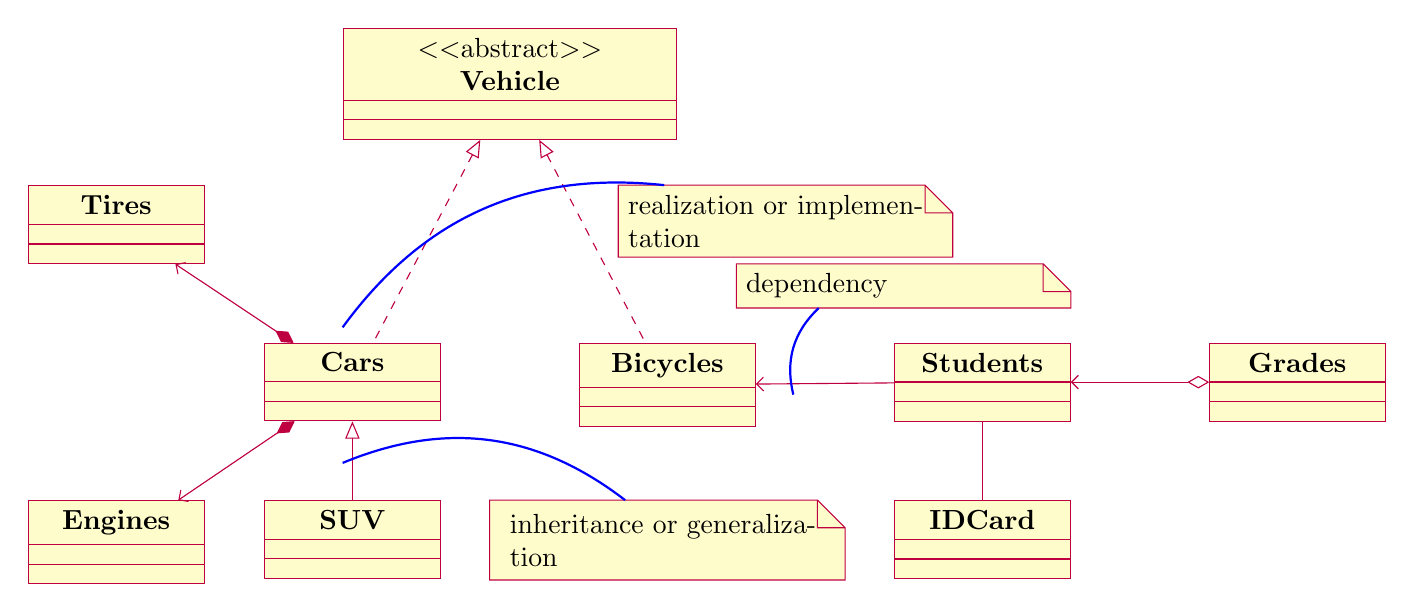
\begin{tikzpicture}[]
    \begin{abstractclass}[text width=4cm]{Vehicle}{0,0}
    \end{abstractclass}

    \umlnote (note1) at (3.5,-2) {realization or implementation};

    \begin{class}[text width=2cm]{Cars}{-2,-4}
    \implement{Vehicle}
    \end{class}

    \begin{class}[text width=2cm]{Bicycles}{2,-4}
    \implement{Vehicle}
    \end{class}

    \begin{class}[text width=2cm]{Students}{6,-4}
    \end{class}
    \unidirectionalAssociation{Students}{}{}{Bicycles}

    \umlnote (note2) at (5,-3) {dependency};
    \node[right=1em of Bicycles] (node2) {};
    \draw[thick,blue] (note2) edge[bend right=30] (node2.south);


    \begin{class}[text width=2cm]{Grades}{10,-4}
    \end{class}

    \aggregation{Grades}{}{}{Students}

    \begin{class}[text width=2cm]{IDCard}{6,-6}
    \end{class}

    \association{Students}{}{}{IDCard}{}{}

    \begin{class}[text width=2cm]{Tires}{-5,-2}
    \end{class}
    \composition{Cars}{}{}{Tires}{}{}

    \begin{class}[text width=2cm]{Engines}{-5,-6}
    \end{class}
    \composition{Cars}{}{}{Engines}{}{}

    \begin{class}[text width=2cm]{SUV}{-2,-6}
        \inherit{Cars}
    \end{class}
    \umlnote[minimum width=4.5cm, minimum height=1.0cm] (note3) at (2.0,-6.0) {inheritance or generalization};

    \node[below=1.5em of Cars] (node3) {};
    \draw[thick,blue] (note3) edge[bend right=30] (node3.north west);

    \node[above=0.2em of Cars] (node1) {};
    \draw[thick,blue] (note1) edge[bend right=30] (node1.west);
\end{tikzpicture}
\end{document}
